% -----------------------------------------------------------------------
% -----------------------------------------------------------------------
\section*{Aufbau}
% Zell: Kapitel 7.1
Es gibt eigentlich historisch gesehen nicht \textit{das} Perzeptron, sondern eine ganze Familie verwandter Modelle neuronaler Netze, die von Frank Rosenblatt Anfang der 60er Jahre entwickelt wurden und die alle mit Perzeptron bezeichnet wurden.

Ein allgemeines Perzeptron hat folgenden Aufbau (Vgl. Abbildung \ref{fig:perzeptron-minsky-papert}):
\begin{itemize}
	\item \emph{Schicht mit Eingabezellen} \\
	Retina - Dient der reinen Datenaufnahme (Muster) und hat festgewichtete Verbindungen zur nächsten Neuronenschicht. (Diese Schicht wird im Folgenden oftmals nicht dargestellt.)
	
	\item \emph{Schicht mit Neuronen} \\
	Eingabeschicht - Neuronen ohne Informationsverarbeitung jedoch mit trainierbaren Verbindungen zum Ausgabeneuron.

	\item Ausgabeneuron $\Omega$ \\
	Klassifikator - Neuron mit Informationsverarbeitung, welches angibt, ob das an der Retina anliegende Muster vom Perzeptron erkannt wird oder nicht.
\end{itemize}

\begin{figure}[ht!] \centering 
	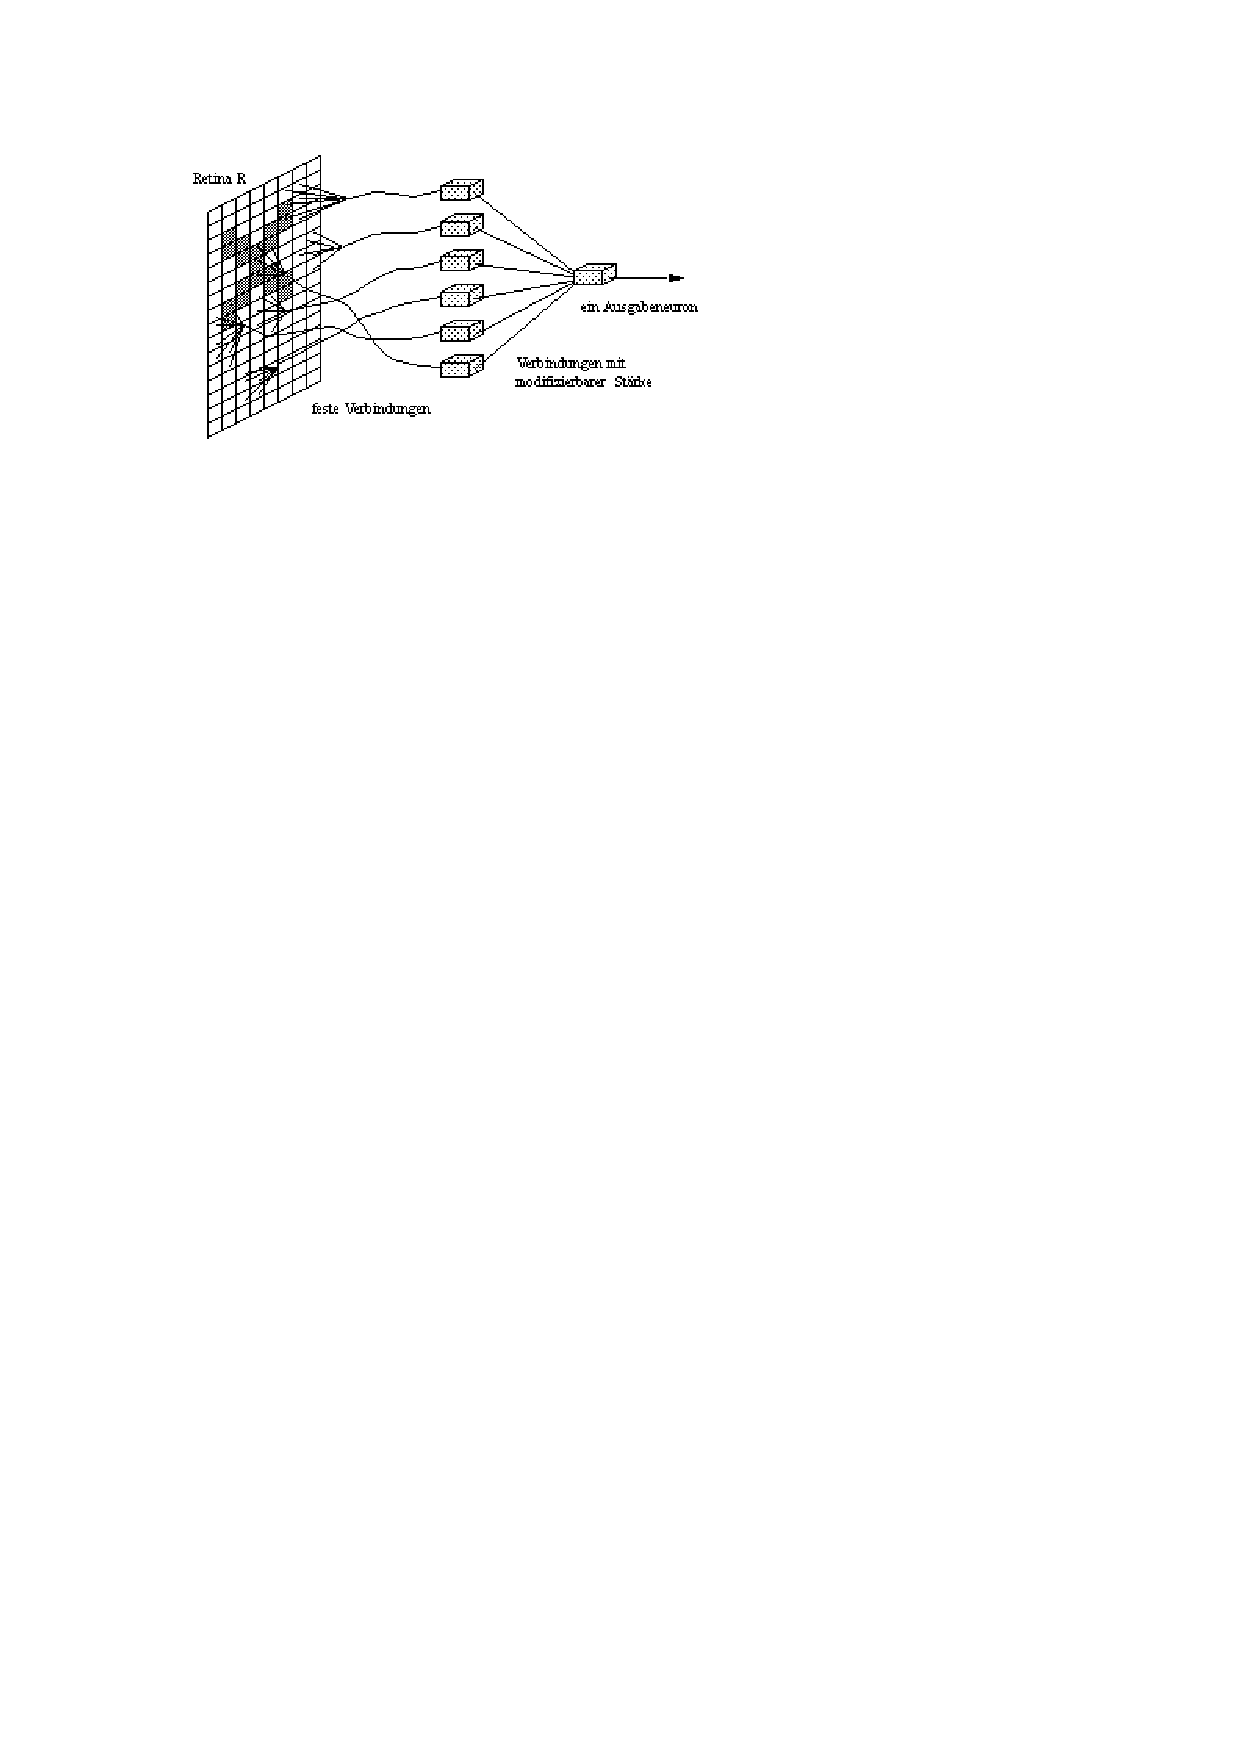
\includegraphics[width=\linewidth]{figures/ch02_perzeptron-minsky-papert.pdf}
	\caption{Struktur des Perzeptron nach Minsky und Papert.}
	\label{fig:perzeptron-minsky-papert}
\end{figure}

Weiterhin wird unter dem Begriff \emph{Perzeptron} oft das binäre Modell des Perzeptrons verstanden, bei dem die Eingaben und die Aktivierungen der Neuronen nur binäre Werte 0 und 1 (bzw. -1 und 1) annehmen dürfen. Die Gewichte können allerdings beliebige reelle Werte annehmen.

% -----------------------------------------------------------------------
\subsection*{Neuronen des Perzeptrons}
% Zell: Kapitel 7.2
Die Neuronen der Eingabeschicht werden in diesem Modell nicht spezifiziert. Es genügt, wenn man sie als \emph{binäre Eingaben} betrachtet.
Damit kann das Schema eines Perzeptrons wie in Abbildung \ref{fig:perzeptron-schema} links dargestellt werden. Dabei ist jedes Neuron der Ebene 0 fest mit allen Neuronen der Eingabeschicht verbunden.

\begin{figure}[ht!] \centering 
	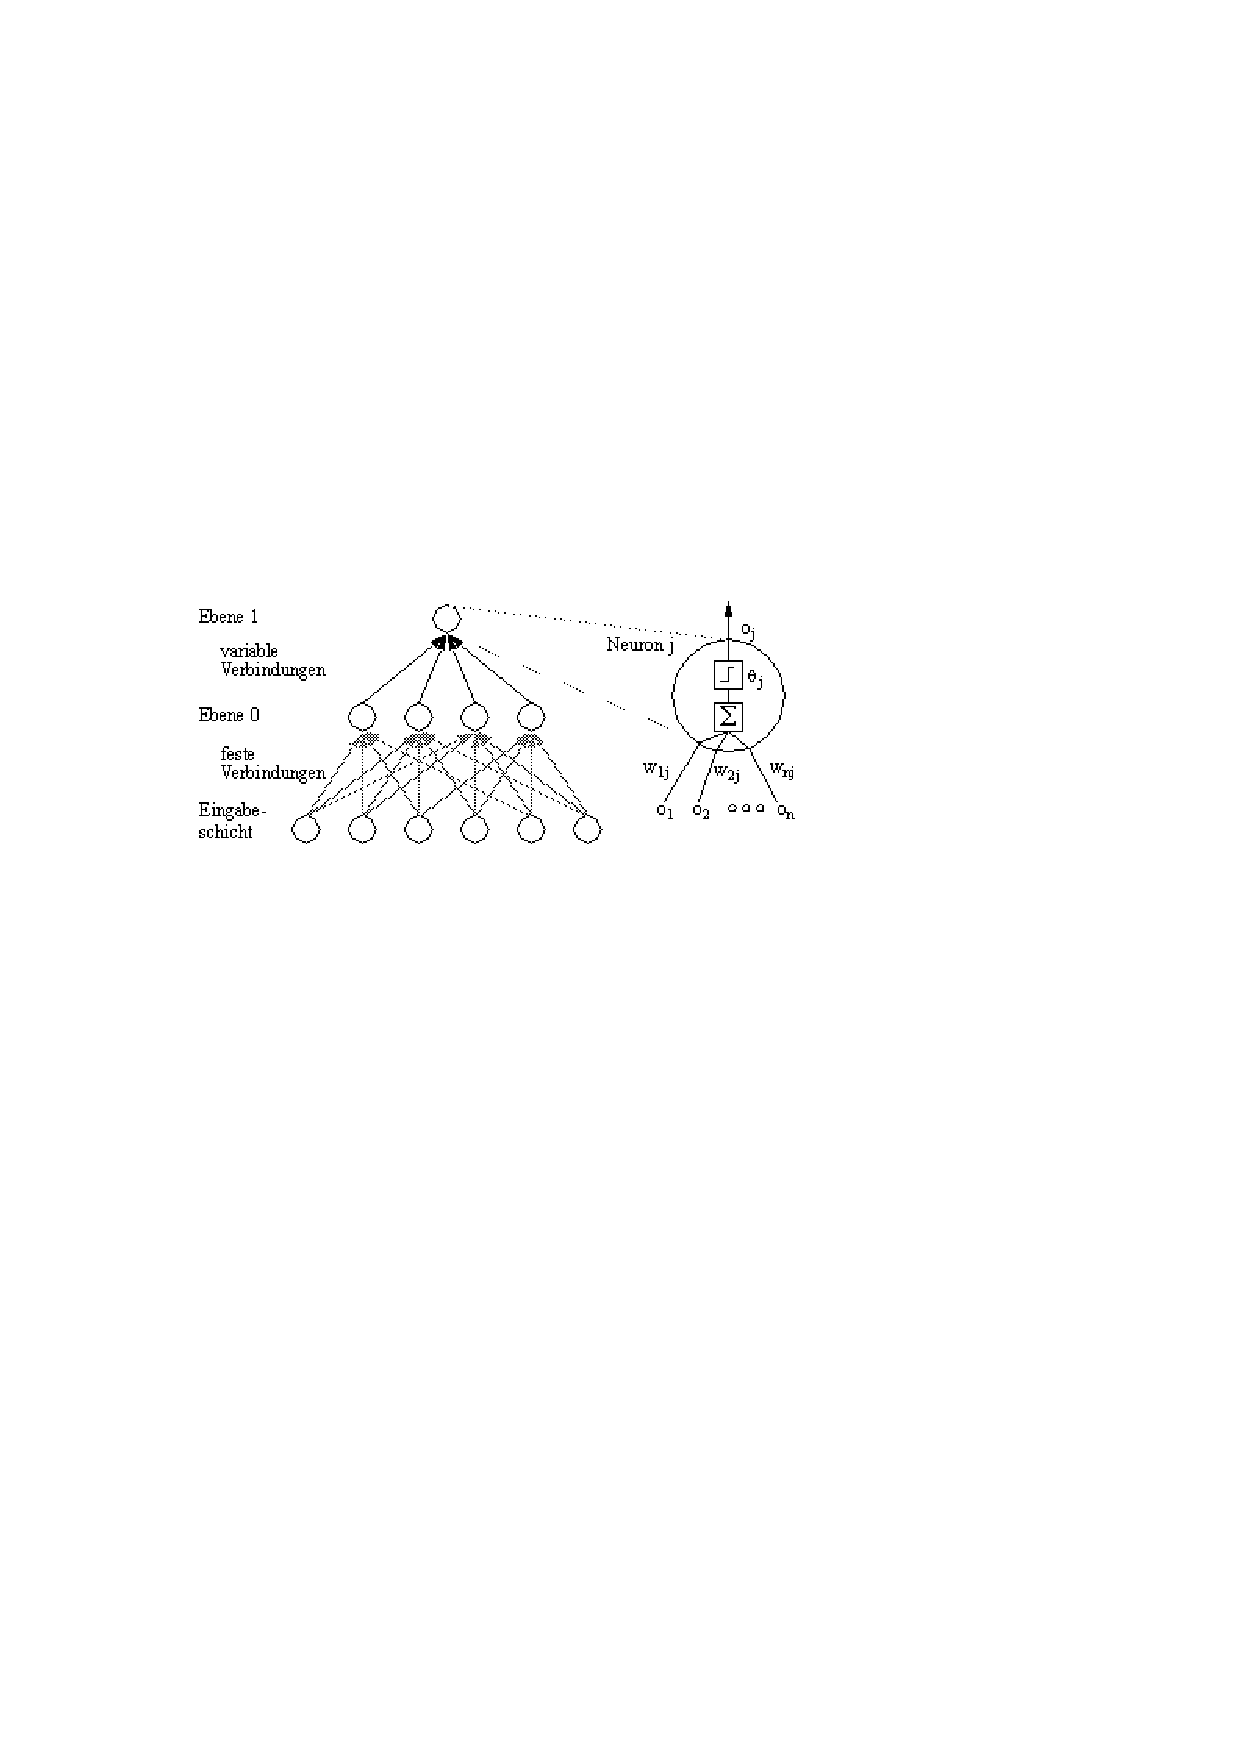
\includegraphics[width=\linewidth]{figures/ch02_perzeptron-schema.pdf}
	\caption{Schema des Perzeptrons (links) und Ausgabeneuron des Perzeptrons (rechts).}
	\label{fig:perzeptron-schema}
\end{figure}

Jedes Neuron der Ebenen 0 und 1 des Perzeptrons hat das in Abbildung \ref{fig:perzeptron-schema} rechts dargestellte Verhalten: Es summiert seine Eingaben auf ($net_j$), die sich als Ausgaben der Vorgängerneuronen ($o_i$) multipliziert mit dem jeweiligen Gewicht $w_{ij}$ ergeben: 
\[
	net_j = \sum_i o_i \cdot w_{ij}
\]

 Auf diese Netzeingabe $net_j$ wird eine binäre Schwellenwertfuktion angewandt: Die Ausgabe $o_j$ ist 1, falls die Netzeingabe größer oder gleich dem Schwellenwert $\theta_j$ ist, andernfalls ist die Ausgabe 0:
\[
	o_j = a_j = 
	\begin{cases}
		1 &\text{falls } net_j \ge \theta_j \\
		0 &\text{sonst}
	\end{cases}
\]

% -----------------------------------------------------------------------
\subsection*{Repräsentierbarkeit und Lernfähigkeit}

\subsubsection*{Repräsentierbarkeit} 
Repräsentierbarkeit bezeichnet die Fähigkeit eines Netzes, eine gegebene Funktion (Prädikat) mit dem neuronalen Netz realisieren zu können. Hierbei ist die Topologie des Netzes vorgegeben, es dürfen aber alle Gewichte und Schwellenwerte korrekt bzw. optimal gewählt werden.

\subsubsection*{Lernfähigkeit} 
Lernfähigkeit ist die Fähigkeit eines Lernalgorithmus, ein Netzwerk eine repräsentierbare Funktion (Prädikat) lernen zu lassen. D.h. die Gewichte und Schwellenwerte durch den \emph{Algorithmus} korrekt zu bestimmen. \\

Die Unterscheidung zwischen Repräsentierbarkeit und Lernfähigkeit ist sehr wichtig\footnote{Die Unterscheidung ist auch aus historischen Gründen sehr wichtig, weil sie in der ersten Blütephase neuronaler Netze noch nicht bekannt war und daher ein berühmtes Theorem, das Perzeptron-Lern-Theorem von F. Rosenblatt über die Fähigkeit des Perzeptron-Lernalgorithmus, meist falsch verstanden wurde.}:
\emph{Repräsentierbarkeit} stellt eine Fähigkeit des Netzes dar und ist nur von der Topologie und den gewählten Aktivierungs- und Ausgabefunktionen des Netzes abhängig, jedoch unabhängig von einem gewählten Lernalgorithmus.
\emph{Lernfähigkeit} hingegen ist eine Eigenschaft eines speziellen Lernalgorithmus. 



% -----------------------------------------------------------------------
% -----------------------------------------------------------------------
\section*{Lineare Trennbarkeit}
% Zell: Kapitel 7.3
Das Konzept der linearen Trennbarkeit kann man am besten an einem einfachen Beispiel, dem bekannten XOR-Problem, demonstrieren. Man betrachte hierzu ein einstufiges Perzeptron-Netzwerk mit einem Ausgabeneuron $j$ in Ebene 1 und zwei Neuronen in Ebene 0. Die Ausgabe des Neurons $j$ soll 0 sein, falls seine binären Eingaben gleich sind ($o_1 = o_2$) sonst soll sie 1 sein. Das heißt, damit $o_j = 1$ ist, muss gelten:
\[
	net_j = o_1 w_{1j} + o_2 w_{2j} \ge \theta_j
\]
Für $w_{2j} \ge 0$ ist dies äquivalent zu der Ungleichung
\[
	o_2 \ge \frac{1}{w_{2j}} ( \theta_j - o_1 w_{1j})
\]
Für einen konstanten Schwellwert $\theta_j$ ergibt sich also eine Gerade in der durch $o_1$ und $o_2$ gebildeten Ebene (siehe Abbildung \ref{fig:lineare-separierbarkeit}). Alle Punkte oberhalb dieser Geraden stellen bei positivem $w_{2j}$ Kombinationen von $o_1$ und $o_2$ dar, für die das Neuron feuert. Bei negativem $w_{2j}$ sind alle Punkte unterhalb der Geraden Punkte, für die das Neuron feuert.

\begin{figure}[ht!] \centering 
	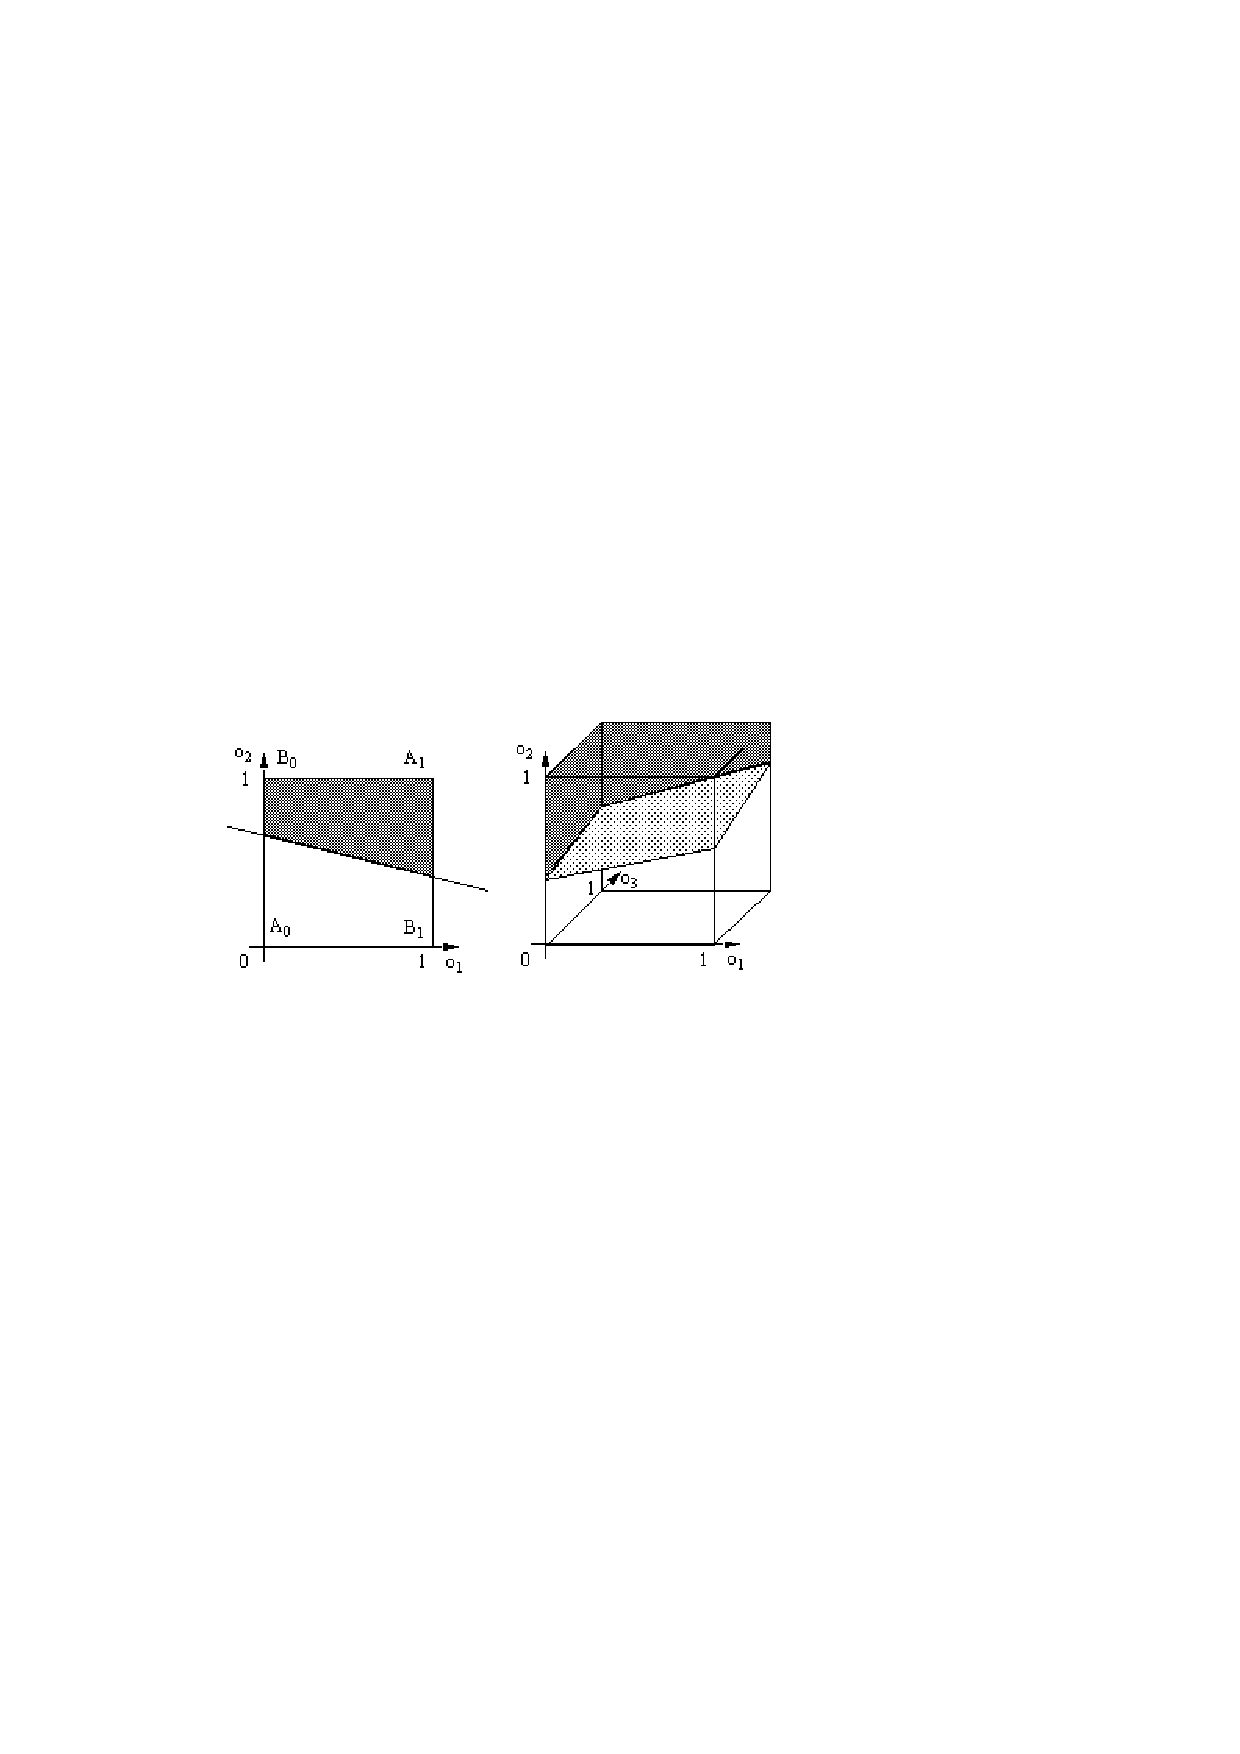
\includegraphics[width=\linewidth]{figures/ch02_lineare-trennbarkeit.pdf}
	\caption{Lineare Trennbarkeit und das XOR-Problem.}
	\label{fig:lineare-separierbarkeit}
\end{figure}

Ein neuronales Netz, welches das XOR-Problem lösen will, muss die Punkte $A_0 (0|0)$ und $A_1 (1|1)$ einer Klasse A zuordnen, die Punkte $B_0 (0|1)$ und $B_1 (1|0)$ der Klasse B. Diese Trennung ist mit einer einzigen Gerade, welche den Eingabereaum linear trennt, nicht möglich. 
Deshalb gilt: Die Menge $A = \{A_0, A_1\}$ und $B = \{B_0, B_1\}$ des XOR-Problems sind nicht linear separierbar, d.h. es gibt keine Wertekombination von $w_{1j}$, $w_{2j}$ und $\theta_j$, für die $net_j < \theta_j$ für alle Punkte in A und zugleich $net_j \ge \theta_j$ für alle Punkte in B ist.

Bei $n$ Eingängen eines Neurons, kann man den Raum der Eingaben als n-dimensionalen Würfel darstellen (sofern die Eingaben auf $[0,1]$ beschränkt ist, sonst ist es der n-dimensionale Raum).
Das Neuron trennt diesen Eingaberaum durch eine $(n-1)$-dimensionale \emph{Hyperebene}. Für $n=3$ ist dies in Abbildung \ref{fig:lineare-separierbarkeit} dargestellt.

Allgemein gilt: Ein einstufiges Perzeptron (d.h. ein Perzeptron mit nur einer Stufe modifizierbarer Gewichte) kann nur linear separierbare Mengen, d.h. Mengen, die durch eine Hyperebene trennbar sind, klassifizieren.


% -----------------------------------------------------------------------
\subsection*{Entscheidungsfunktion $g(x)$}
Eine Entscheidungsfunktion weißt einem Eingabevektor $\vec{x}$ eine der $k$ Klassen zu. Diese Klasse wird als $C_k$ bezeichnet.
Es seien folgende Werte gegeben:
\begin{align*}
	& \vec{x} = (x_1, \ldots, x_n)^T &\text{Merkmalsvektor} \\
	& \vec{w} = (w_1, \ldots, w_n)^T &\text{Gewichtsvektor} \\
	& w_0	&\text{Bias/Threshold}
\end{align*}

\subsubsection*{Zwei Klassen}
Bei $k=2$ gilt die einfachste Form der Entscheidungsfunktion $g(x)$:
\[
	g(\vec{x}) = \sum_{i=1}^{n} w_i x_i + w_0 = \vec{w}^T \vec{x} + w_0
\]
Der Merkmalsvektor $\vec{x}$ wird der Klasse $C_1$ zugeordnet wenn $g(\vec{x}) \ge 0$, andernfalls wird er der Klasse $C_2$ zugeordnet. Die Entscheidungsfunktion $g(x)$ gibt den Abstand zwischen Entscheidungsgrenze und Merkmalsvektor zurück. 

Die Entscheidungsgrenze ist damit für $g(\vec{x}) = 0$ definiert. Sie entspricht einer $(d-1)$-dimensionalen Hyperebene innerhalb eines $d$-dimensionalen Merkmalsraums und wird mit $H$ bezeichnet:
\[
	H: g(\vec{x}) = \sum_{i=1}^{n} w_i x_i + w_0 = \vec{w}^T \vec{x} + w_0 = 0
\]
Der normierte Vektor $\vec{w}$ gibt die Richtung und der Bias $w_0$ die Lage dieser Entscheidungsgrenze an. Die Hyperebene $H$ trennt den Merkmalsraum in zwei Hälften auf; Entscheidungsregion $R_1$ für $C_1$ und $R_2$ für $C_2$. Liegt $\vec{x}$ in $R_1$ ($g(x) \ge 0$), zeigt auch der Normalenvektor $\vec{w}$ in $R_1$. Abbildung \ref{fig:lineare-entscheidunsfunktion} zeigt dies. Für den Abstand $r$ zwischen Hyperebene $H$ und Merkmalsvektor $\vec{x}$ gilt:
\[
	r = \frac{g(x)}{||w||}
\]

\begin{figure}[ht!] \centering 
	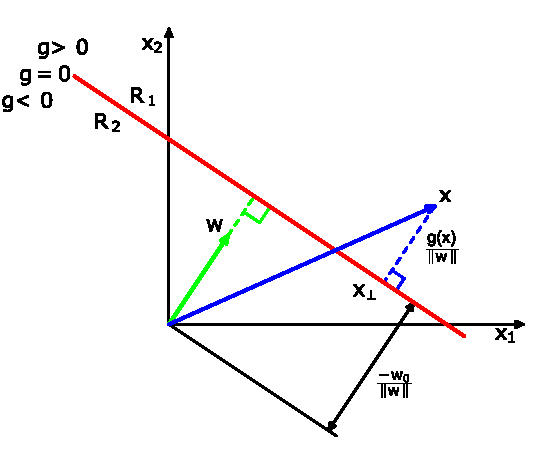
\includegraphics[width=\linewidth]{figures/ch02_lineare-entscheidungsfunktion.pdf}
	\caption{Grafisches Schaubild zur linearen Entscheidungsfunktion $g(x)$ in einem zweidimensionalen Merkmalsraum.}
	\label{fig:lineare-entscheidunsfunktion}
\end{figure}


\subsubsection*{Mehrere Klassen}
Bei $k > 2$ Klassen gibt es verschiedene Möglichkeiten eine k-Klassen-Diskriminantfunktion durch Kombinationen von Zwei-Klassen-Diskriminantfunktionen zu bestimmen:
\begin{itemize}
 	\item \emph{one-versus-the-rest} \\
 	$k-1$ Klassifikatoren die alle jeweils ein Zwei-Klassen-Problem lösen: Sie trennen Punkte, die zur Klasse $C_k$ gehören von Punkten, die nicht zu $C_k$ gehören (siehe Abbildung \ref{fig:lineare-entscheidungsfunktion-mehrere-klassen} oben).

 	\item \emph{one-versus-one} \\
 	Bei diesem Ansatz gibt es $\frac{k(k-1)}{2}$ binäre Diskriminantfunktionen: Eine für jedes mögliche Klassenpaar (siehe Abbildung \ref{fig:lineare-entscheidungsfunktion-mehrere-klassen} unten). 
 \end{itemize} 

\begin{figure}[ht!] \centering 
	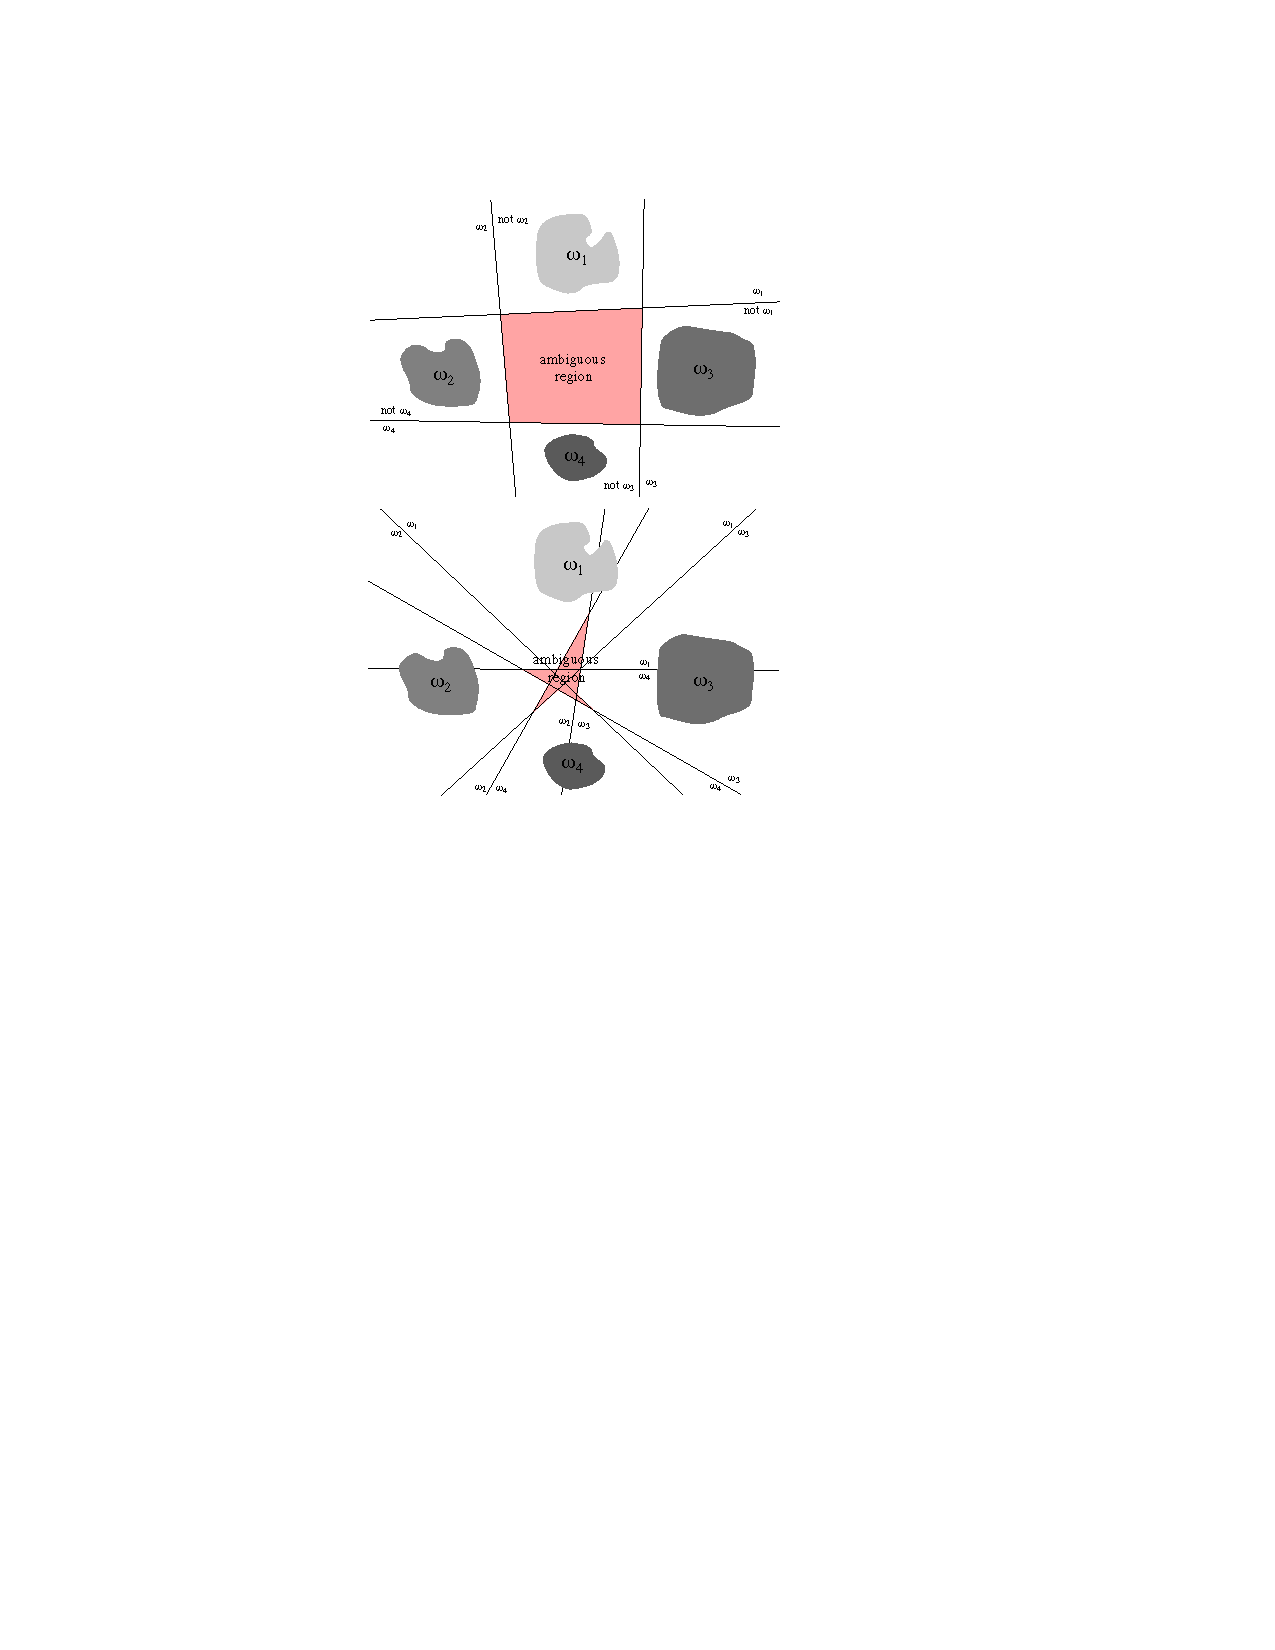
\includegraphics[width=\linewidth]{figures/ch02_lineare-entscheidungsfunktion-mehrere-klassen.pdf}
	\caption{Lineare Entscheidungsgrenzen für ein 4-Klassen-Problem. Oben der \emph{one-versus-the-rest} Ansatz ($C_i$ oder nicht $C_i$). Unten der \emph{one-versus-one} Ansatz ($C_i$ oder $C_j$ für alle $j \ne i$)}
	\label{fig:lineare-entscheidungsfunktion-mehrere-klassen}
\end{figure}

Beide Vorgehensweisen führen jedoch zu Bereichen des Merkmalsraums, welche nicht eindeutig einer Klasse zugeordnet werden können (in Abbildung \ref{fig:lineare-entscheidungsfunktion-mehrere-klassen} farbig hervorgehoben).
Deshalb wird für den Fall dass $k > 2$ ist der Ansatz der Entscheidungsfunktion für zwei Klassen wie folgt erweitert:
\[
	g_k(\vec{x}) = \vec{w}_k^T\vec{x} + w_{k0}
\]
Der daraus resultierende Klassifikator wird \emph{linear machine} genannt und teilt den Merkmalsraum in $k$ Entscheidungsregionen auf (siehe Abbildung \ref{fig:linear-machine}. Dabei ist $g_k(\vec{x})$ die größte Diskriminante, wenn $x$ in der Region $R_k$ liegt. Demnach wird der Merkmalsvektor $\vec{x}$ der Klasse $C_k$ zugeordnet, wenn gilt:
\[
	g_k(\vec{x}) > g_j(\vec{x}) \qquad \text{für alle } j \ne k
\]
Die Entscheidungsgrenze zwischen Klasse $C_k$ und Klasse $C_j$ ist gegeben für $g_k(\vec{x}) = g_j(\vec{x})$. Daraus folgt, analog zur Entscheidungsgrenze für den Zwei-Klassen-Fall, eine $(d-1)$-dimensionale Hyperebene, für die gilt:
\[
	(\vec{w}_k - \vec{w}_j)^T x + (w_{k0} - w_{j0}) = 0
\]
Im Gegensatz zur Entscheidungsgrenze im Zwei-Klassen-Fall ist hier nicht der Gewichtsvektor $\vec{w}$ entscheidend, sondern die Differenz $\vec{w}_k - \vec{w}_j$.

\begin{figure}[ht!] \centering 
	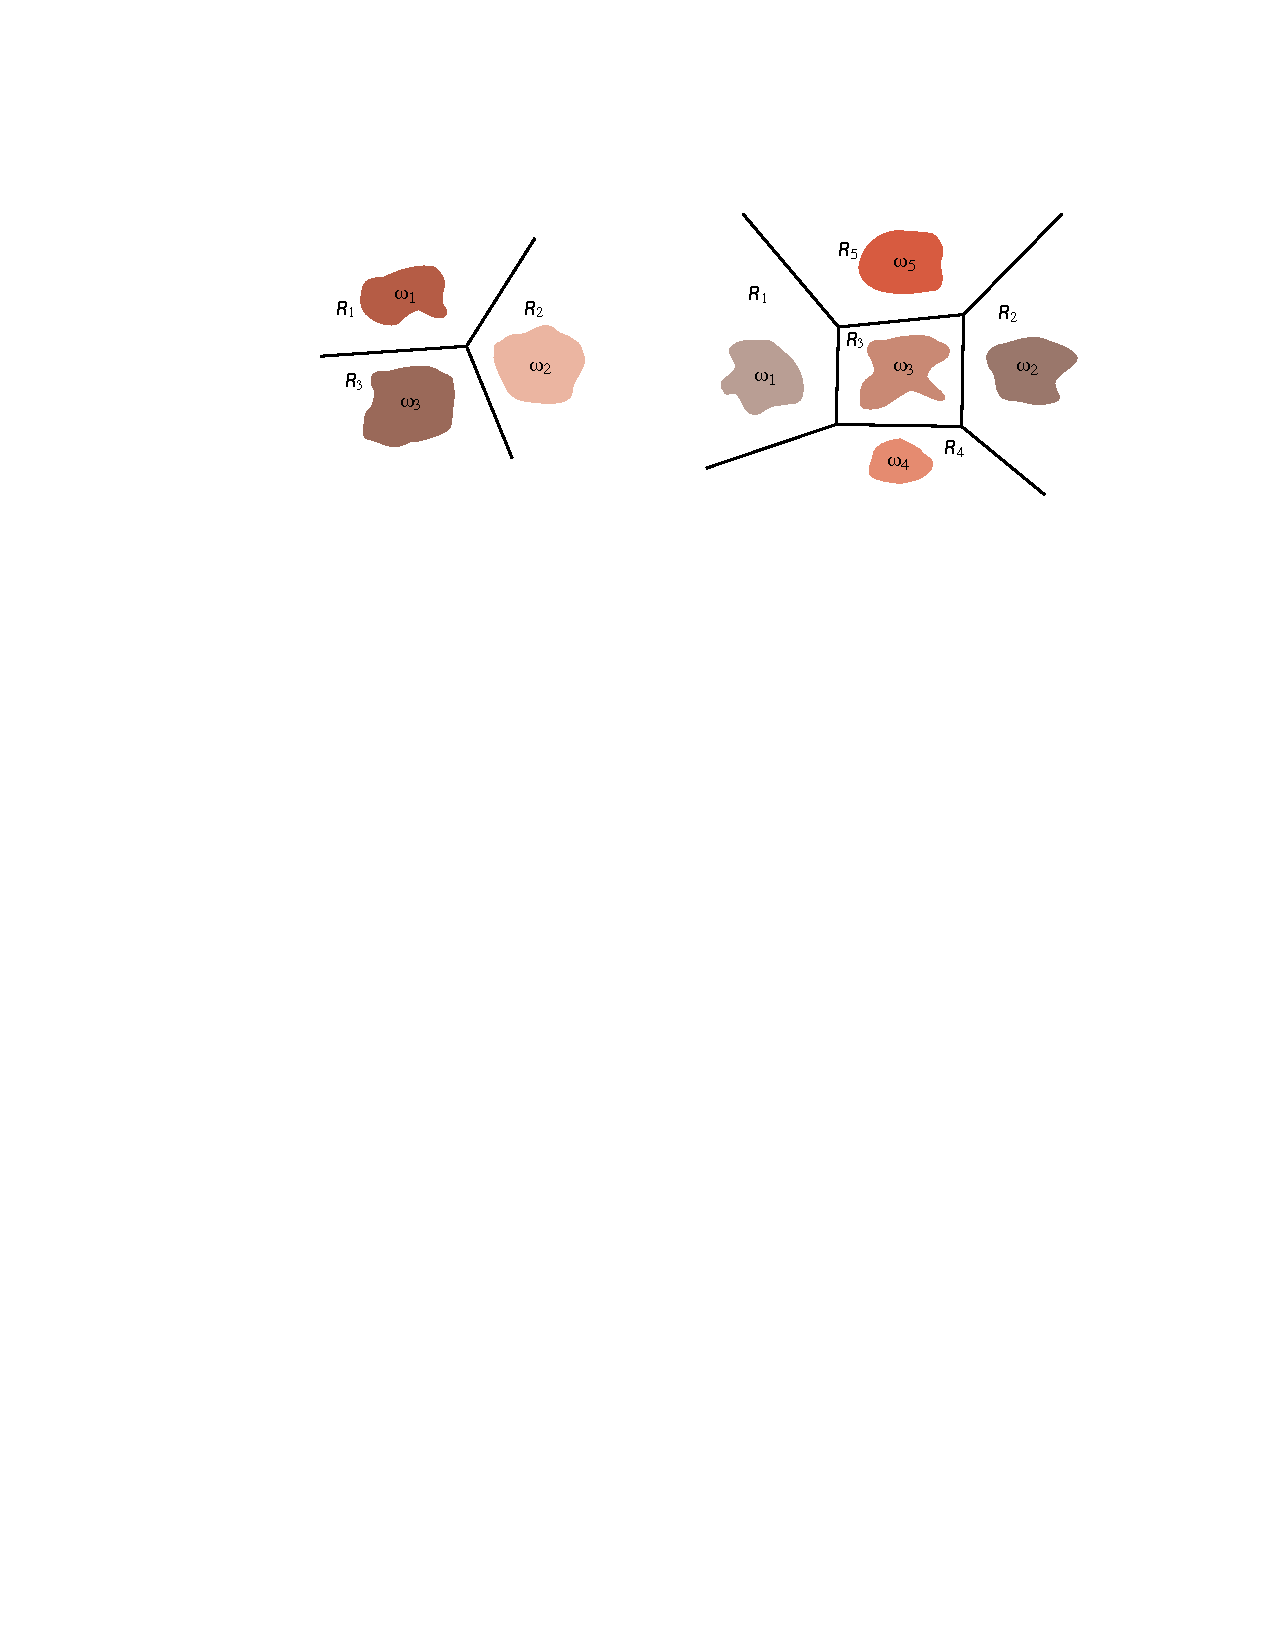
\includegraphics[width=\linewidth]{figures/ch02_linear-machine.pdf}
	\caption{Entscheidungsgrenzen erzeugt von einer \emph{linear machine} für ein Drei-Klassen- und ein Fünf-Klassen-Fall.}
	\label{fig:linear-machine}
\end{figure}


\subsubsection*{Least Squares}
ToDo

\subsubsection*{Fisher's linear discriminant}
ToDo


% -----------------------------------------------------------------------
% -----------------------------------------------------------------------
\section*{Multilayer-Perceptron (MLP)}
% -----------------------------------------------------------------------
\subsection*{Zweistufiges Perzeptron}
% Zell: Kapitel 7.4
Zweistufige binäre Perzeptrons sind mächtiger als einstufige, sie können konvexe Polygone klassifizieren. Dazu berechnen die Neuronen der ersten Ebene Hyperebenen wie im vorigen Fall auch, diese können dann aber in der zweiten Ebene durch ein Neuron, welches ein logisches AND durchführt, zum Schnitt gebracht werden, sodass sich ein konvexes Polygon ergibt.

Abbildung \ref{fig:perzeptron-zweistufig} zeigt ein Beispiel für ein zweistufiges Perzeptron und ein typisches Gebiet, dessen Punkte als Eingabe in das neuronale Netz aktzeptiert werden.

\begin{figure}[ht!] \centering 
	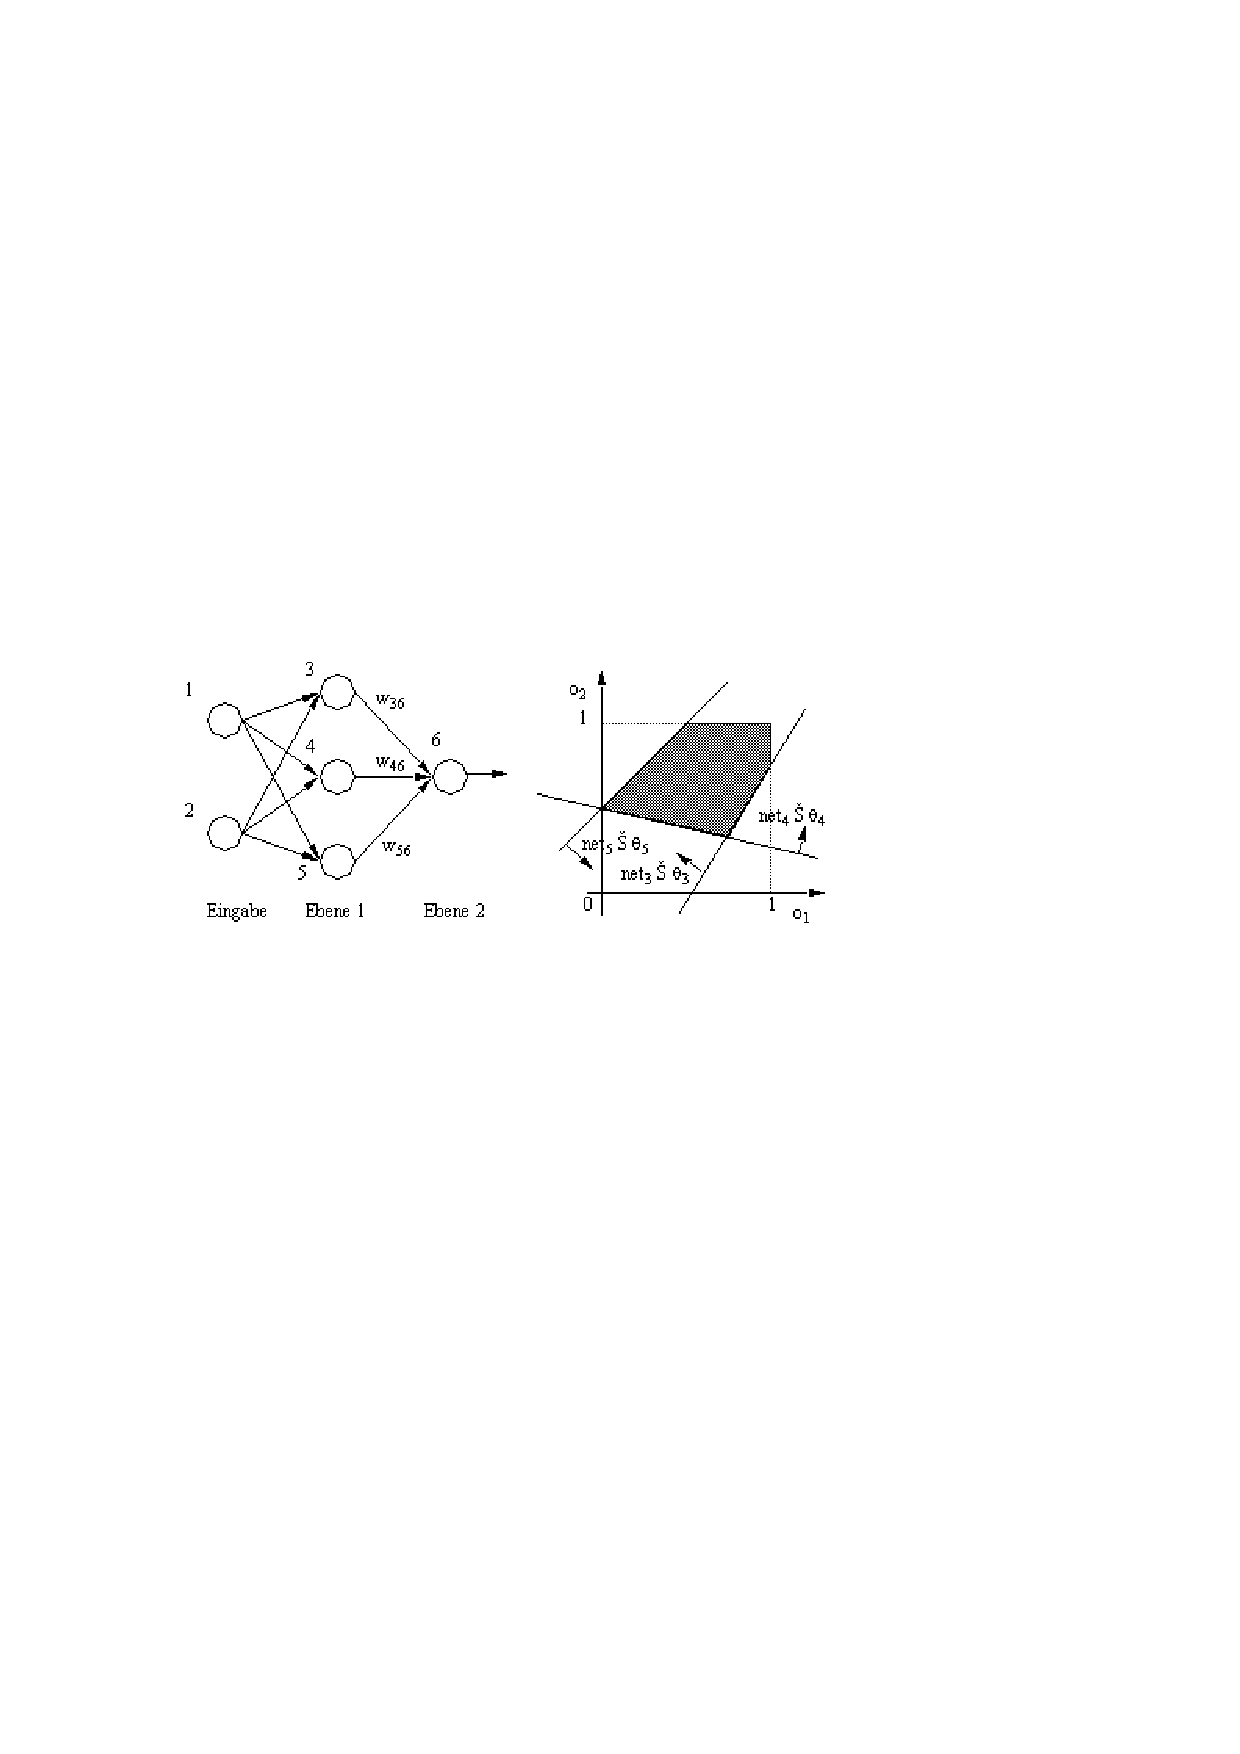
\includegraphics[width=\linewidth]{figures/ch02_perzeptron-zweistufig.pdf}
	\caption{Zweistufiges Perzeptron und ein von ihm akzeptiertes Gebiet im Merkmalsraum.}
	\label{fig:perzeptron-zweistufig}
\end{figure}

Die Funktion des logischen \emph{AND} kann dadurch erreicht werden, dass das Ausgangsneuron einen Schwellenwert besitzt, welcher der Summe der Gewichte der Verbindungen in dieses Neuron entspricht bzw. geringfügig kleiner ist:
Neuron 6 in Abbildung \ref{fig:perzeptron-zweistufig} führt durch $w_{36} = w_{46} = w_{56} = \frac{1}{3}$ und $\theta_6 = 0.9$ ein logisches AND\footnote{Die Verknüpfung der Gebiete ist nicht auf AND beschränkt. Sie könnte ebenfalls durch eine andere logische Funktion (z.B. OR, NAND, ...), welche sich mit einem einstufigen Perzeptron darstellen lässt, realisiert werden.} auf seine Eingabe durch. So wird $o_6 = 1$ genau dann, wenn $(o_1, o_2)$ im dunkel markierten konvexen Polygon liegt.

% -----------------------------------------------------------------------
\subsection*{Dreistufiges Perzeptron}
% Zell: Kapitel 7.5
Dreistufige binäre Perzeptrons können durch Überlagerung und Schnitt konvexer Polygone Mengen beliebiger Form repräsentieren. Abbildung \ref{fig:perzeptron-dreistufig} zeigt auch hierfür ein Beispiel.

\begin{figure}[ht!] \centering 
	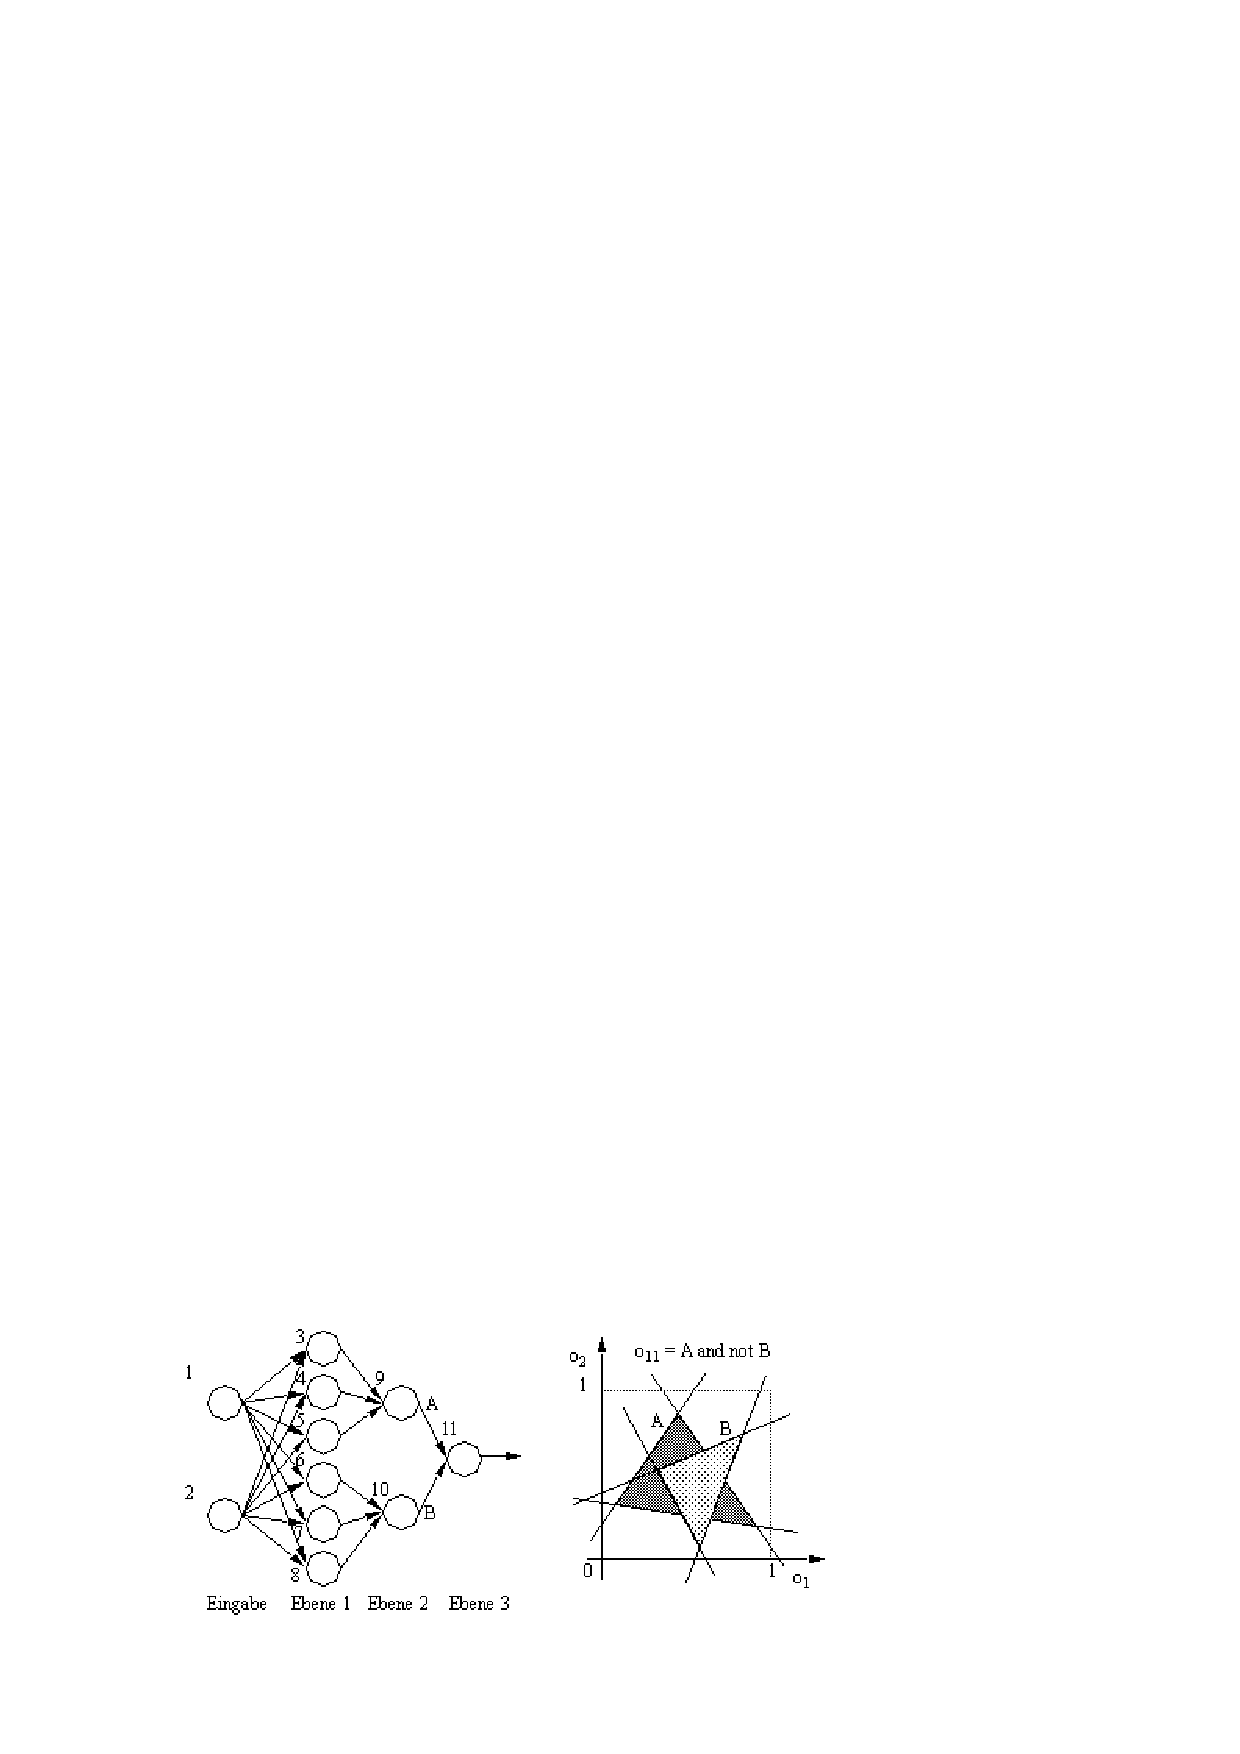
\includegraphics[width=\linewidth]{figures/ch02_perzeptron-dreistufig.pdf}
	\caption{Dreistufiges Perzeptron und ein von ihm akzeptiertes Gebiet im Merkmalsraum.}
	\label{fig:perzeptron-dreistufig}
\end{figure}

Weitere Stufen besitzen in diesem Modell keine zusätzliche Fähigkeiten mehr.


% -----------------------------------------------------------------------
% -----------------------------------------------------------------------
\section*{Lernverfahren}
Unter einem \emph{Lernverfahren} versteht man einen Algorithmus, der dem Neuronalen Netz beibringt, für einen gegebenen Merkmalsvektor $\vec{x}$ den erwarteten Wert $t$ am Ausgang $o$ zu produzieren. Ist $o = t$, dann hat das Netz erfolgreich gelernt.

Um ein Neuronales Netz zu trainieren werden dessen Gewichte angepasst. Sie \textit{speichern} das Wissen des Netzes. Diese Gewichte werden während der Traingsphase laufend angepasst. Abbildung \ref{fig:perzeptron-learning} zeigt den schematischen Lernprozess eines Perzeptrons.

\begin{figure}[ht!] \centering 
	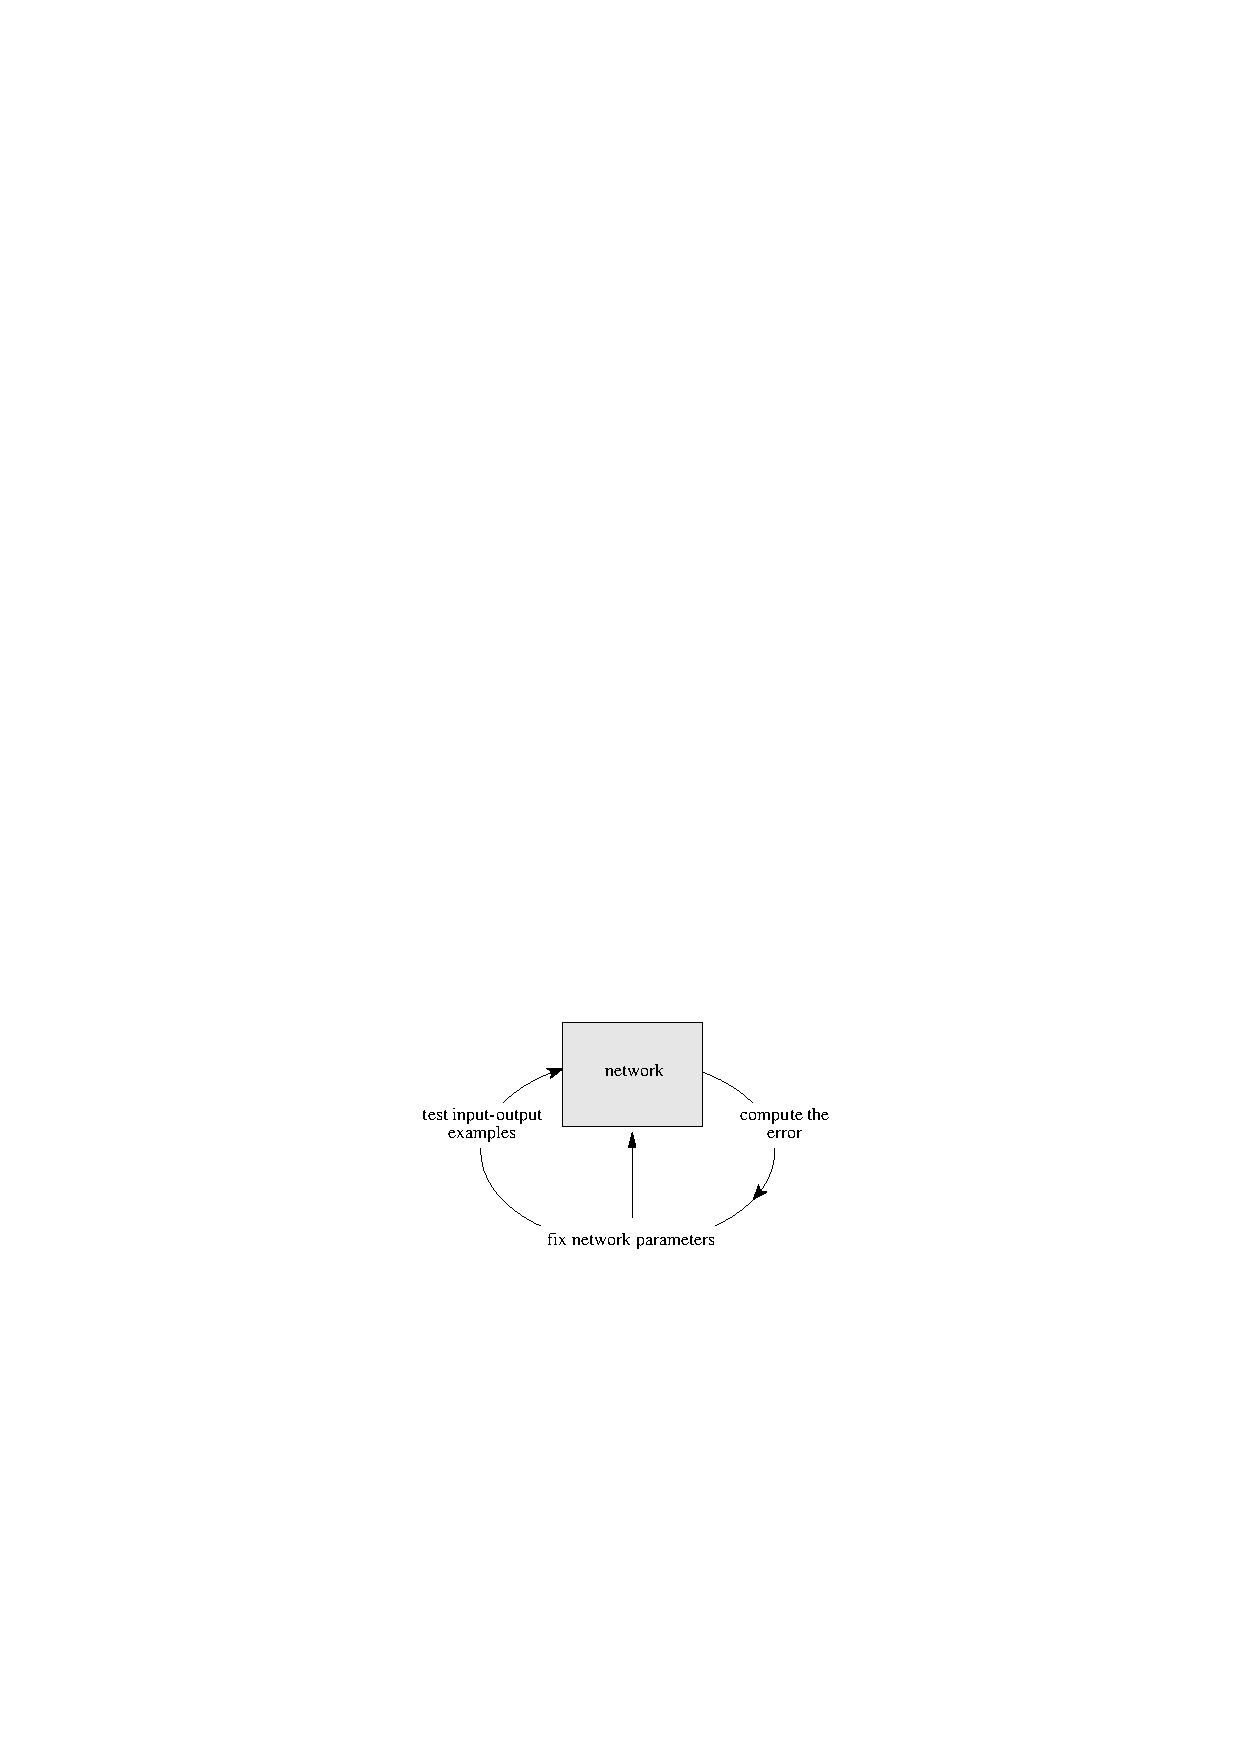
\includegraphics[width=\linewidth]{figures/ch02_perzeptron-learning.pdf}
	\caption{Schematischer Lernprozess eines Neuronalen Netzes.}
	\label{fig:perzeptron-learning}
\end{figure}

Man unterscheidet zwei Klassen von Lernalgorithmen:
\begin{itemize}
	\item \emph{überwachte Methoden} - Beim überwachten Lernen wird jedem Merkmalsvektor ein erwartetes Ergebnis zugeordnet. Lernalgorithmen beobachten die Abweichung zwischen berechnetem und erwartetem Ergebnis. Die Gewichte werden entsprechend der Größe der Abweichung angepasst. Ein solches Verfahren wird deshalb auch als \emph{Learning with a teacher} bezeichnet.
	\item \emph{unüberwachte Methoden} - Beim unüberwachten Lernen ist der genaue Ausgabewert, welcher aufgrund eines Merkmalsvektors berechnet werden soll, sowie die Anzahl und Lage der Cluster innerhalb des Merkmalsraums unbekannt. Die Trainingsmenge besteht lediglich aus Eingabemustern. Das Netzwerk muss deshalb selbst (und ohne "`teacher"') in der Lage sein, eine Klassifikation vorzunehmen. \\
	Z.B.: \emph{Self organizing maps} (SOMs)
\end{itemize}

Das \emph{überwachte} Lernen wird weiter in zwei Kategorien unterteilt:
\begin{itemize}
	\item \emph{reinforcement learning} - Hier ist nach jeder Berechnung der Ausgabe nur bekannt, ob das Netz das korrekte Ergebnis liefert oder nicht. Aufgrund dieser Informationen werden die Gewichte angepasst. Hier kann \emph{nur der Merkmalsvektor} für die Gewichtsanpassung verwendet werden.
	\item \emph{error correction} - Beim Lernen mit error correction ist die Gewichtsänderung vom Merkmalsvektor \emph{und} der Stärke der Abweichung zum gewünschten Ausgabwert abhängig.
\end{itemize}

\subsection*{Hebbsche Lernregel}
Die \emph{Hebbsche Lernregel} ist die älteste und einfachste Lernregel für Neuronale Netze. Sie besagt, dass das Gewicht zwischen zwei Einheiten dann verändert wird, wenn beide gleichzeitig aktiv sind:
\[
	\Delta w_{ij} = \eta \cdot a_i \cdot o_j
\]
Dabei ist $\Delta w_{ij}$ die Gewichtsänderung von Neuron $i$ zu Neuron $j$, $\eta$ die Lernrate, welche den Grad der Änderung bestimmt, $a_i$ die Aktivierung von Neuron $i$ und $o_j$ die Ausgabe von Neuron $j$, welches mit Neuron $i$ verbunden ist.

\subsection*{Perzeptron Lernalgorithmus}
Der Perzeptron Lernalgorithmus basiert auf der Hebbschen Regel. Gegeben ist eine Menge markierter Daten:
\[
	(x,t) \in X \times \{0,1\}
\]
Gesucht werden jene Gewichte $\hat{w}$, für die das Perzeptron alle Daten korrekt zuordnet.

Der Algorithmus berechnet für jeden Merkmalsvektor $x$ der Datenmenge $X$ die Ausgabe $o_x$ des Perzeptrons als gewichtete Summe der einzelnen Merkmale $x_j$:
\[
	o_x = \varphi(w \cdot x) = \varphi( \sum_{j=0}^{m} w_j x_j)
\]
Dabei ist $\varphi$ die Aktivierungsfunktion des Perzeptrons und $m$ die Dimension des Merkmalsraumes\footnote{Mit Bias-Trick ist $m = \text{Dimension Merkmalsraum} + 1$.}

Für das Anpassen der Gewichte gilt dann:
\begin{align*}
	&w_{t+1} =
	\begin{cases}
		w_{t} &\text{wenn } o_x = t_x \\
		w_{t} - x &\text{wenn } o_x = 1 \text{ und } t_x = 0\\
		w_{t} + x &\text{wenn } o_x = 0 \text{ und } t_x = 1
	\end{cases} \\
	&\text{alternativ auch geschrieben als:} \\
	&w_{t+1} = w_{t} + (t_x - o_x) x
\end{align*}
Wobei $w_{t}$ das aktuelle und $w_{t+1}$ das neue Gewicht ist. Entspricht die Ausgabe $o_x$ dem erwarteten Wert $t_x$, bleibt das Gewicht unverändert. Ist $o_x = 1$, sollte aber $0$ sein, wird der Merkmalsvektor abgezogen (Gewicht wird vermindert). Ist $o_x = 0$, sollte jedoch $1$ sein, wird er hinzuaddiert (Gewicht wird erhöht).
Dieser Trainingsvorgang wird so lange wiederholt, bis das Perzeptron alle Daten korrekt klassifiziert hat und damit $\hat{w}$ gefunden wurde.

Der Perzeptron Lernalgorithmus konvergiert in endlicher Zeit, wenn die Trainingsdaten linear separierbar sind (\emph{Perzeptron-Konvergenz-Theorem}). Damit kann das Perzeptron in endlicher Zeit all das lernen, was es repräsentieren kann.

Es handelt sich dabei um einen Lernalgorithmus des \emph{überwachten Lernens} mit Verstärkung (\emph{reinforcement learning}).

\subsubsection*{Pocket Perceptron Algorithm}
Ist ein Problem nicht linear separierbar, terminiert der Perzeptron Algorithmus nicht. In vielen Fällen ist es jedoch ausreichend, bei nicht pefekt linear separierbaren Problemen davon auszugehen, dass diese linear separierbar sind, weil die meisten Punkte im Merkmalsraum trotzdem richtig klassifiziert werden.
Hierfür gibt es eine Variante des Perzeptron Algorithmus: Den \emph{Pocket Perceptron Algorithm}. Dieser geht prinzipiell genau so vor wie der normale Perzeptron Algorithmus. Er merkt sich jedoch den bisher besten Gewichtsvektor.\footnote{Der beste Gewichtsvektor wird in die "`Tasche"' gesteckt. Daher der Name des Algorithmus.} Am Ende bleibt so jener Gewichtsvektor übrig, welcher am wenigsten Beispiele falsch klassifiziert.

\subsection*{Delta-Regel}
Die Delta-Regel (auch \emph{Widrow-Hoff-Regel} genannt) beruht auf dem Vergleich zwischen der gewünschten Ausgabe $t_{\Omega}$ und der tatsächlich beobachteten Ausgabe $o_{\Omega}$ eines Ausgabeneurons bzw. der tatsächlich beobachteten Aktivierung $a_{\Omega}$\footnote{Abhängig davon, ob im Teaching Input $t_{\Omega}$ die gewünschte \emph{Aktivierung} oder die gewünschte \emph{Ausgabe} hinterlegt ist.}:
\begin{align*}
	&\delta = t_{\Omega} - o_{\Omega} \\
	&\delta = t_{\Omega} - a_{\Omega}
\end{align*}
Wie auch bei der Hebbschen Lernregel gibt es drei Fälle zu unterscheiden (die beobachtete Aktivität ist zu hoch oder zu niedrig, oder entspricht dem gewünschten Ergebnis). Deshalb lautet die Formel der Delta-Regel wie folgt:
\[
	\Delta w = \eta \delta o_{\Omega}
\]
Bei der Delta-Regel ist die Gewichtsänderung aller Gewichte zu einem Ausgabeneuron $\Omega$ proportional zur Differenz der aktuellen Aktivierung $a_{\Omega}$ bzw. Ausgabe $o_{\Omega}$ und dem dazugehörigen Teaching Input $t_{\Omega}$.  

Die Delta-Regel gilt damit nur für SLPs, da sich die Formel immer auf den Teaching Input $t_{\Omega}$ bezieht und für innere Verarbeitungsschichten von Neuronen kein Teaching Input existiert. Sie wird deshalb mit dem Backpropagation-Algorithmus verallgemeinert.


\subsection*{Online- und Offline-Learning}
Der Lernvorgang kann \emph{online} und \emph{offline} erfolgen:
\begin{itemize}
	\item \emph{Online Learning} - Beim Online Learning werden die Gewichte nach jedem Beispiel aus den Trainingsdaten angepasst. Dieses Vorgehen zeichnet sich durch \emph{Schnelligkeit} aus.
	\item \emph{Offline Learning} - Beim Offline Learning hingegen werden die Gewichte nach eine Menge von Trainingsbeispielen verändert. Weshalb dieses Verfahren auch \emph{Batch-Trainingsverfahren} genannt wird, da ein Stapel Ergebnisse auf einmal korrigiert wird. Ein solcher Trainingsabschnitt wird als \emph{Epoche} bezeichnet. Dieses Vorgehen zeichnet sich durch \emph{Stabilität} aus.
\end{itemize}

\subsection*{Wichtige Fragen zum Lernen}
Fragen, über die man sich beim Lernen Gedanken machen sollte, sind im Folgenden aufgeführt.
\begin{itemize}
	\item Woher kommt die Lerneingabe und in welcher Form liegt sie vor?
	\item Wie werden die Gewichte modifiziert, um möglichst schnell und sicher zu lernen?
	\item Wie kann der Erfolg eines Lernprozesses objektiv gemessen werden?
	\item Kann ermittelt werden, welches das beste Lernverfahren ist?
	\item Kann vorhergesagt werden, ob ein Lernverfahren in endlicher Zeit terminiert?
	\item Wie wird das Gelernte im Netz gespeichert?
	\item Kann verhindert werden, dass neu gelernte Muster alte erlernte Assoziationen wieder zerstören? (\emph{Stabilitäts-Plastizitäts-Dilemma})
\end{itemize}
Diese Fragen können nicht allgemein beantwortet werden, sondern müssen für jedes Lernverfahren und jede Topologie von Netzwerk neu diskutiert werden.



% -----------------------------------------------------------------------
% -----------------------------------------------------------------------
\section*{Fehlerfunktionen}
Ein Neuronales Netz zu \emph{trainieren} heißt die Kostenfunktion (engl. cost function), also die Fehler des Netzes zu \emph{minimieren}.
Der zeitliche Verlauf des Fehlers wird als sogenannte \emph{Lernkurve} aufgetragen. Die Motivation für die Erschaffung dieser Lernkurve liegt darin, dass man mit ihr darstellen kann, ob das Netz Fortschritte macht oder nicht. Dabei sollte der Fehler normiert sein, also ein Abstandsmaß zwischen richtiger und aktueller Ausgabe des Netzes darstellen.

Man unterscheidet zwei Arten von Fehlern:
\begin{itemize}
	\item \emph{Spezifischer Fehler} $Err_p$ - Er wird über ein einziges Trainingsbeispiel, also \emph{online}, gebildet.
	\item \emph{Gesamtfehler} $Err$ - Er wird über alle Trainingsbeispiele einer Epoche, also \emph{offline}, gebildet.
\end{itemize}
Daher gilt bei $P$ Trainingsbeispielen in einer Epoche folgender Zusammenhang:
\[
	Err = \sum_{p \in P} Err_p
\]

\subsection*{Mean Squared Error (MSE)}
Der Mean-Squared-Error berechnet den spezifischen Fehler $Err_p$ anhand der quadrierten Differenz zwischen erwarteter und tatsächlicher Ausgabe.
\[
	Err_p = \frac{1}{2} \sum_{\Omega \in O} ( t_{\Omega} - o_{\Omega})^2
\]
Dabei ist $\Omega$ eines von $O$ Ausgabeneuronen. Der Vorfaktor von $\frac{1}{2}$ dient der vereinfachten Ableitung der Gleichung.

\subsection*{Euklidischer Abstand}
Der spezifische Fehler basierend auf dem euklidischen Abstand berechnet sich wie folgt.
\[
	Err_p = \sqrt{ \sum_{\Omega \in O} ( t_{\Omega} - o_{\Omega})^2 }
\]

\subsection*{Root-Mean-Square (RMS)}
Der Root-Mean-Square wird allgemein häufig verwendet, weil er auf grobe Ausreißer mehr Rücksicht nimmt.
\[
	Err_p = \sqrt{ \frac{
		\sum_{\Omega \in O} ( t_{\Omega} - o_{\Omega})^2 }
		{|O|}
		}
\]

\subsection*{Gewichtsänderung}
Die Gewichtsänderung $\Delta w$ ist proportional zur Ableitung des Fehlers nach den Gewichten. Es gilt:
\[
	\Delta w \sim - \nabla Err(w)
\]
Mit $\eta$ als Proportionalitätskonstante wir daraus:
\[
	\Delta w = - \eta \nabla Err(w)
\]
Die Ableitung der Fehlerfunktion nach den Gewichten wird im Folgenden als partielle Ableitung nach einem Gewicht $w_{i,\Omega}$ geschrieben. Umgangssprachlich formuliert wird damit an jedem Gewicht gedreht und die Änderung (Ableitung) der Fehlerfunktion betrachtet. Damit erhält man die Information $\Delta w_{i,\Omega}$, welche sagt wie das Gewicht verändert werden soll.
\[
	\Delta w_{i,\Omega} = - \eta \frac{\partial Err(w)}{\partial w_{i,\Omega}}
\]
